\documentclass{article}
\usepackage[a4paper, margin=20mm]{geometry}
\usepackage{graphicx}
\usepackage{float}
\usepackage{subfigure}
\usepackage{amsmath}
\usepackage{amsfonts}
\title{Practical Submission Sheet}
\newcommand{\bb}[1]{\textbf{#1}}
\newcommand{\ol}[1]{\overline{#1}}
\date{}
\begin{document}
	\maketitle
	\begin{tabular}{ll}
		\bb{Term}: 2020-1 & \bb{Submission Date}: \today\\
		\bb{Lecture Date}: October 2nd, 2020. & \bb{Practical Number}: 6\\
		\bb{Course Code}: PHY249 & \bb{Section}: G2903\\
		\bb{Registration Number}: 11912610 & \bb{Roll No}: 03\\
		\bb{Student Name}: Aayush Arya & \\
	\end{tabular}
	
	\section*{Aim} Minimize the boolean expressions below and implement the truth table using an AOI logic.
	\begin{itemize}
		\item[(i)] $Z = A.B + A\cdot(B+C) + B.(B+C)$
		\item[(ii)] $Z = [A.\overline{B}.(C+B.D) + \overline{A}.\overline{B}].C$
		\item[(iii)] $f = (x+\overline{x}.\overline{y}).(\overline{x}+\overline{y}) + y.z$
	\end{itemize}
	\section*{Concepts Learnt}
	Learnt how certain properties in boolean algebra help us relate digital logic with a special field and some properties that arise from that. Learnt how powerful these properties are when it comes to simplifying boolean expressions.	
	
	\section*{Key Observations \& Insights}
	Expressions (i), (ii) and (iii) reduce to\\
	(i) $Z = B + A\cdot C$\\
	(ii) $Z = \ol{B} \cdot C$\\
	(iii) $f = \ol{y} + y.z$\\
	
	\section*{Application Areas}
	
	Using this approach, several complicated digital circuits can be condensed significantly and is thus useful in digital electronics. The idea due to the generality of the mathematics can be extended anywhere boolean expressions are involved.
	\section*{Report}
	There are certain laws of boolean algebra that are always followed

	\begin{align*}
A+B &= B + A \\
A \cdot B &= B\cdot A \tag{Commutative law}\\
A + ( B+ C) & = (A+B)+C\\
A\cdot(B \cdot C) &= (A \cdot B) \cdot C \tag{Associative law}\\
A\cdot(B+C) & = A \cdot B + A\cdot C \tag{Distributive Law}\\
	\end{align*}
	In fact, if we define $\mathbb{F}_2= \{0,1\}$, where 0 and 1 represent identity elements with respect to addition and multiplication respectively, the set $
	\mathbb{F}_2$ along with the opearations of addition and multiplication, form a finite field, given that the multiplication and addition rules are defined as 
	$$ A+B := (A+B)\mod(2) $$
	$$ A\cdot B := AB \mod(2)$$	
	
	where $A$, $B$ $\in \mathbb{F}_2$\\
	
	And several important properties that are followed in digital systems can be derived from merely these assumptions alone. Some of these are 
	\begin{align*}
	 A \cdot 0&=0\\
	 A \cdot 1&=A\\
	 A+0&=A\\
	 A+1 &= 1\\
	 A+A &= A\\
	 A+\ol{A} & = 1\\
	 A.A &= A\\
	 A.\ol{A} & = 0\\
	 \ol{\ol{A}} & = A\\
	\end{align*}
	
	We will use some of these in the following text without reference. These properties help us to find links between different logic systems, as well as to simplify some logic circuits. \\
	
	Expression (i) can be simplified as the following
	
	\begin{align*}
	 Z & = A\cdot B + A\cdot(B+C) + B\cdot(B+C)\\
	  & = (A\cdot B) + (A\cdot B) + A\cdot C + B\cdot B + B\cdot C\\
	  & = A\cdot B + A\cdot C + B + B\cdot C\\
	  & = (A+1)\cdot B + A\cdot C + B\cdot C\\
	  & = B + B\cdot C + A\cdot C\\
	  & = B\cdot (1+C) + A\cdot C\\
	  Z & = B + A\cdot C \tag{1}\\
	\end{align*}
	
	The truth table for the logic system represented by equation (1) was written down
	 
		\begin{table}[H]
		\centering
		\begin{tabular}{|l|l|l|l|}
			\hline
			Input A & Input B & Input C & Output\\
			\hline
			0 & 0 & 0 & 0\\
			0 & 0 & 1 & 0\\
			0 &1 &0& 1\\
			0 & 1 & 0 & 1\\
			0 &1 & 1 & 1\\
			1 & 0 & 0 & 0\\
			1 &0 & 1 &1\\
			1 &1 &0 &1\\
			1 &1 &1 &1\\
			\hline
		\end{tabular}
		\caption{Truth table for the logic system $Z = B + A\cdot C$.}
	\end{table}

	An AOI gate combination was simulated as depicted in Figure 1 and the truth table was then verified empirically.
	\begin{figure}[H]
		\centering
		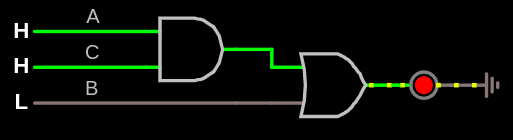
\includegraphics[width=0.75\textwidth]{one}
		\caption{Circuit diagram for an AOI logic satisfying truth table 1.}
		\label{circuit1}
	\end{figure}

	In a similar fashion, expression (ii) can be reduced to
	
	\begin{align*}
	Z & = [A\cdot\overline{B} \cdot(C + B\cdot D) + \overline{A} \cdot \overline{B}]\cdot C\\
	 & = [A\cdot\overline{B}\cdot C + A\cdot B \cdot B \cdot D + \overline{A} \cdot \overline{B}]\cdot C\\
	 & = A\cdot \ol{B} \cdot C \cdot C + A \cdot \ol{B} \cdot B \cdot D \cdot C + \ol{A} \cdot\ol{B} \cdot C\\
	 & = A\cdot\ol{B} \cdot C + 0 + \ol{A}\cdot\ol{B} \cdot C\\
	 & = (A+\ol{A})\cdot\ol{B}\cdot C\\
	 & = 1 \cdot \ol{B} \cdot C\\
	Z & = \ol{B} \cdot C \tag{2}
	\end{align*}
	
	It is very well worth noting that A the inputs A and D are redundant and the required circuit needs just two inputs. An AOI logic system can be constructed straightforwardly by inverting the input B and constructing an AND gate with $\ol{B}$ and C as the inputs, as shown below.
	
	\begin{figure}[H]
		\centering
		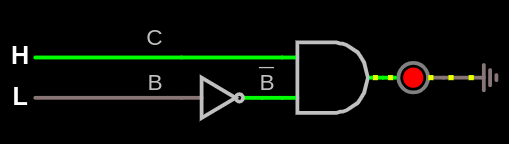
\includegraphics[width=0.75\textwidth]{two}
		\caption{AOI logic circuit corresponding to the expression $ Z = \ol{B}\cdot C$}
		\label{circuit2}
	\end{figure}
	
	The truth table for this logic system is 
	
			\begin{table}[H]
		\centering
		\begin{tabular}{|l|l|l|}
			\hline
			Input B & Input C & Output\\
			\hline
			0 & 0 & 0\\
			0 & 1 & 1\\
			1 & 0 & 0\\
			1 & 1 & 0\\
			\hline
		\end{tabular}
		\caption{Truth table for the logic system $Z = \ol{B}\cdot C$.}
	\end{table}
And finally, for expression (iii),
 \begin{align*}
  f &= (x+\ol{x}.\ol{y}). (\ol{x} + \ol{y}) + y. z\\
   & = (x. \ol{x} + x.\ol{y} + \ol{x}.\ol{x}.\ol{y} + x. \ol{y}.\ol{y} + y. z)\\
   & = 0 + x. \ol{y} + \ol{x}.\ol{y} + x.\ol{y} + y. z\\
   & = x.\ol{y} + \ol{x}.\ol{y} + y.z\\
   & = (x+\ol{x}).\ol{y}+ y.z\\
   & = 1.\ol{y} + y.z\\
   f & = \ol{y} + y.z \tag{3}\\
 \end{align*}
   
 Again, it is worth noting that input $x$ is redundant. A circuit diagram for this logic system using AOI gates is shown in Figure 3.
 
 	\begin{figure}[H]
 	\centering
 	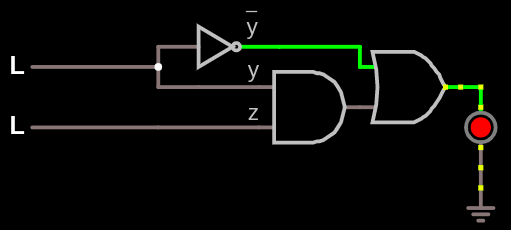
\includegraphics[width=0.75\textwidth]{three}
 	\caption{Circuit diagram for the logic system $f=\ol{y} + y.z$}
 	\label{circuit3}
 \end{figure}

  The truth table that was verified was the following
 
 		\begin{table}[H]
 	\centering
 	\begin{tabular}{|l|l|l|l|}
 		\hline
 		Input y & Input z & Output\\
 		\hline
 		0 & 0 & 1\\
 		0 & 1 & 1\\
 		1 & 0 & 0\\
 		1 & 1 & 1\\
 		\hline
 	\end{tabular}
 	\caption{Truth table for the logic system $f = \ol{y} + y.z$.}
 \end{table}

\end{document}}